\begin{frame}[t]{Хистология на нервната тъкан}
    В нервната тъкан има два основни вида клетки - неврони и глиоцити.
    Електрични импулси се предават по невроните, а (невро-)глията, 
    както понякога се нарича съвкупността от глиоцити, подпомага тяхната работа.

    От нервна тъкан е изградена нервната система, която се дели на централна (гръбначен мозък и главен мозък) и периферна (соматична и автономна).

\end{frame}

\begin{frame}[t]{Невроглия}
    Глиоцитите могат да участват в митоза, т.е. да се делят. "Най-важните" видове невроглия са:
    \begin{enumerate}
        \item Астроцити - връзка между невроните и кръвта
        \item Олигодендроцити - покриват аксоните на невроните в централната нервна система, образувайки миелинова обвивка, която действа като диелектрик
        \item Шванови клетки - подобни на олигодендроцитите, но в периферната нервна система
        \item Радиална глия - отговарят за неврогенезата и синаптичната пластичност
        \item Микроглия - имунна защита
    \end{enumerate}
\end{frame}

\begin{frame}[t]{Неврони}
    Невроните не участват в митоза. Функционално могат да се разделят на три типа
    \begin{enumerate}
        \item Аферентни (рецептори) - носят информация за околния свят 
        \item Интернерврони (конектори) - свързват различни региони на мозъка, позволяват рефлексите и обучението 
        \item Еферентни (моторни) - активират мускули и жлези
    \end{enumerate}
\end{frame}

\begin{frame}[t]{Хистология на нервната тъкан}
    \begin{figure}[htbp!]
      \centering
      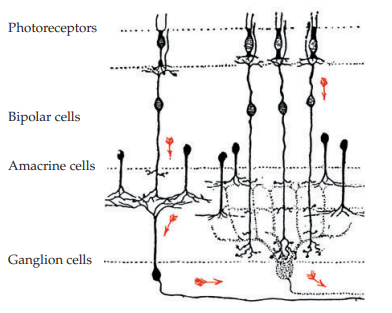
\includegraphics[width=\textwidth,height=0.7\textheight,keepaspectratio]{neuron-complex.PNG}
      \caption{Структура и връзки между клетките на ретината при бозайници. Фиг 1.2 от From Neuron to Brain}
    \end{figure}
\end{frame}

\begin{frame}[t]{Хистология на нервната тъкан}
    \begin{figure}[htbp!]
      \centering
      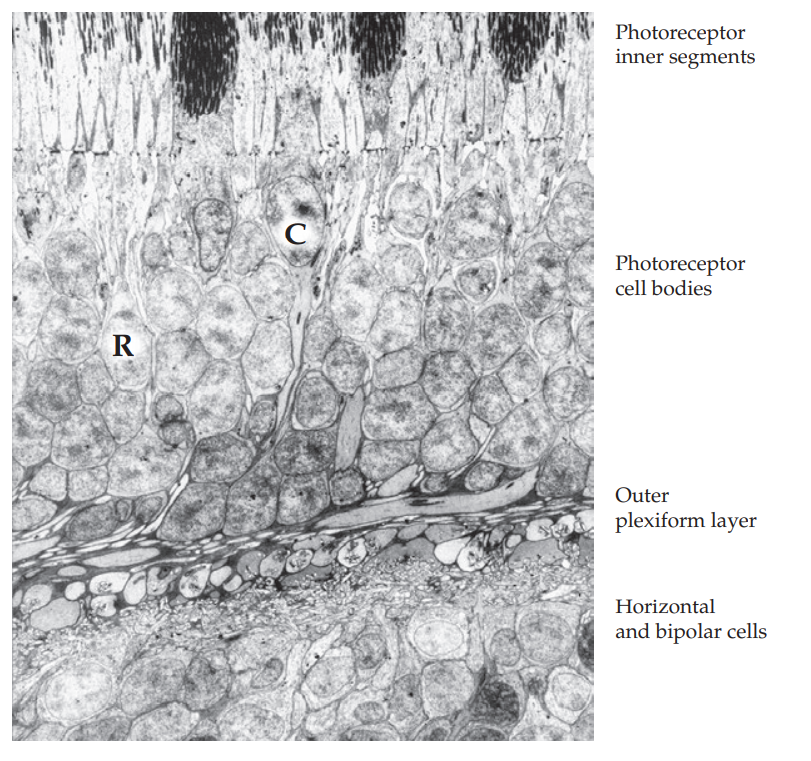
\includegraphics[width=\textwidth,height=0.7\textheight,keepaspectratio]{neurons-macaque.PNG}
      \caption{Електромикроскопска снимка на ретина на макак. Фиг 1.3 от From Neuron to Brain}
    \end{figure}
\end{frame}

